\section{Wannier functions}\label{sec:3.6}

A set of Wannier functions depends on a choice of gauge, and asking for the most localized set fixes it. The interpolation they allow is exact when the Hamiltonian has finite range in their basis, and every quantity interpolated with them must be built in one gauge. We follow Refs.~\cite{marzari1997maximally,souza2001maximally,marzari2012maximally}.

\subsection{From Bloch states to localized orbitals}

Take first a single band $n$ that is separated from all others by gaps throughout the zone. Its $N$ Bloch states each spread over the whole crystal with the same weight in every cell. A superposition of them with phases that add up in one cell and cancel elsewhere is a wave packet localized near that cell:
\begin{equation}
  w_n(\vect{r} - \vect{R}) = \frac{1}{\sqrt N}\sum_{\vect{k}}\ee^{-\ii\vect{k}\cdot\vect{R}}\,\psi_{n\vect{k}}(\vect{r}) ,
  \label{eq:3.6-wannier1}
\end{equation}
with the sum over the $N$ crystal momenta of the Born--von Karman grid, \cref{eq:3.1-kgrid}. The left side is written as a function of $\vect{r} - \vect{R}$ because it is one: Bloch's theorem in the form $\psi_{n\vect{k}}(\vect{r}) = \ee^{\ii\vect{k}\cdot\vect{R}}\psi_{n\vect{k}}(\vect{r} - \vect{R})$ turns the right side into $N^{-1/2}\sum_{\vect{k}}\psi_{n\vect{k}}(\vect{r} - \vect{R})$, the function for $\vect{R} = 0$ shifted by $\vect{R}$. All the Wannier functions of a band are copies of one function, one per cell. The transform inverts with the lattice sum. On the grid of \cref{eq:3.1-kgrid} the same geometric sums that proved \cref{eq:3.1-latticesum} give $\sum_{\vect{k}}\ee^{\ii\vect{k}\cdot\vect{R}} = N\delta_{\vect{R},0}$ for lattice vectors of one Born--von Karman crystal. Multiplying \cref{eq:3.6-wannier1} by $N^{-1/2}\ee^{\ii\vect{k}\cdot\vect{R}}$, summing over $\vect{R}$ and using this identity to collapse the sum over crystal momenta,
\begin{equation}
  \psi_{n\vect{k}}(\vect{r}) = \frac{1}{\sqrt N}\sum_{\vect{R}}\ee^{\ii\vect{k}\cdot\vect{R}}\,w_n(\vect{r} - \vect{R}) .
  \label{eq:3.6-inverse}
\end{equation}
This is the Bloch sum of \cref{eq:3.2-blochsum}, with the Wannier function in place of the atomic orbital. Unlike atomic orbitals, Wannier functions are orthonormal. Writing $w_{n\vect{R}}$ for $w_n(\vect{r} - \vect{R})$,
\begin{equation*}
  \langle w_{n\vect{R}}|w_{n'\vect{R}'}\rangle = \frac1N\sum_{\vect{k}\vect{k}'}\ee^{\ii\vect{k}\cdot\vect{R} - \ii\vect{k}'\cdot\vect{R}'}\langle\psi_{n\vect{k}}|\psi_{n'\vect{k}'}\rangle
  = \frac1N\sum_{\vect{k}}\ee^{\ii\vect{k}\cdot(\vect{R} - \vect{R}')}\,\delta_{nn'} = \delta_{\vect{R}\vect{R}'}\delta_{nn'} .
\end{equation*} The overlap matrix of the tight-binding problem, \cref{eq:3.2-HS}, is then the identity. The normalization of \cref{eq:3.2-bloch} gives $w_n$ the dimension $\Omega^{-1/2}$, the same as $u_{n\vect{k}}$, and a function localized within a few cells has a norm that does not depend on the size of the crystal.

A Bloch state is defined only up to a phase, and $\psi_{n\vect{k}} \to \ee^{\ii\theta_n(\vect{k})}\psi_{n\vect{k}}$ describes the same physical state at every $\vect{k}$. It changes the Wannier function, however, since \cref{eq:3.6-wannier1} adds the states with new relative phases. In the periodic gauge of \cref{eq:A.5-periodic}, with $\theta_n(\vect{k} + \vect{G}) = \theta_n(\vect{k})$, the summand $\psi_{n\vect{k}}(\vect{r})$ at fixed $\vect{r}$ is a periodic function of $\vect{k}$. The value of $w_n$ in cell $\vect{R}$ is then a Fourier coefficient of that function, and its decay with $|\vect{R}|$ is set by how smooth the function is. If $\theta_n$ jumps at random from one $\vect{k}$ to the next, as the phases of a numerical diagonalization do, the sum is a random walk and $w_n$ spreads over the whole crystal. If the periodic parts $u_{n\vect{k}}$ are smooth, the Wannier function decays faster than any power of $|\vect{R}|$, and if they are analytic in a strip of half-width $1/\xi_W$ around the real $\vect{k}$ axis it decays as $\ee^{-|\vect{R}|/\xi_W}$. In two and three dimensions such an analytic choice exists if and only if the Chern invariants of the bands vanish~\cite{brouder2007exponential}. A Chern invariant is a topological integer of a group of bands, a count of how often the phases of its Bloch states must wind across a plane of the zone, and it vanishes in every crystal with time-reversal symmetry, silicon among them.

A single isolated band is the exception. The four valence bands of silicon touch at $\mathrm{\Gamma}$, where three of them are degenerate (\cref{sec:3.3}), and cross elsewhere; no one of them is smooth across the zone. Their sum, the projector $P(\vect{k}) = \sum_{n=1}^{4}|u_{n\vect{k}}\rangle\langle u_{n\vect{k}}|$ on the four-dimensional space they span, is smooth, since the group is separated from the conduction bands by the gap at every $\vect{k}$. Instead of one Wannier function per band, we build $N_W$ functions for the whole group of $N_W$ bands, mixing the bands at each $\vect{k}$ with a unitary $N_W\times N_W$ matrix:
\begin{equation}
  w_n(\vect{r} - \vect{R}) = \frac{1}{\sqrt N}\sum_{\vect{k}}\ee^{-\ii\vect{k}\cdot\vect{R}}\,\psi^W_{n\vect{k}}(\vect{r}), \qquad
  \psi^W_{n\vect{k}} = \sum_m U_{mn}(\vect{k})\,\psi_{m\vect{k}} ,
  \label{eq:3.6-wannier}
\end{equation}
which is the convention of \cref{eq:A.5-wannier}. The gauge matrix $U(\vect{k})$ is periodic, $U(\vect{k} + \vect{G}) = U(\vect{k})$; the phases $\ee^{\ii\theta_n(\vect{k})}$ are its diagonal special case. The rotated states $\psi^W_{n\vect{k}}$ are still Bloch functions at $\vect{k}$, but they are no longer eigenstates of $H_{\mathrm{e}}$, and $n$ is no longer a band index: it labels a Wannier function. Translations, the inverse transform and orthonormality carry over from the single band, with $\psi^W$ in place of $\psi$. Since a unitary mixing within the group leaves $P(\vect{k})$ unchanged, the $N_W$ Wannier functions of a cell, together with their copies in all other cells, span exactly the states of the group~\cite[Eqs.~(8)--(10)]{marzari2012maximally}.

A first smooth gauge comes from projection. Choose $N_W$ trial orbitals $\varphi^{\mathrm{tr}}_n(\vect{r})$ located where the Wannier functions are expected, such as $sp^3$ hybrids on the atoms of silicon or Gaussians at the bond centers, and compute the $N_W\times N_W$ matrix $A^{\mathrm{pr}}_{mn}(\vect{k}) = \langle\psi_{m\vect{k}}|\varphi^{\mathrm{tr}}_n\rangle$. Its L\"owdin orthonormalization
\begin{equation}
  U(\vect{k}) = A^{\mathrm{pr}}(\vect{k})\,\bigl[A^{\mathrm{pr}\dagger}(\vect{k})A^{\mathrm{pr}}(\vect{k})\bigr]^{-1/2} ,
  \label{eq:3.6-projection}
\end{equation}
is unitary, and it is smooth in $\vect{k}$ because the trial orbitals are localized~\cite[Eqs.~(16) and (17)]{marzari2012maximally}. The arbitrary phases of the $\psi_{m\vect{k}}$ cancel in \cref{eq:3.6-projection}: a phase on $\psi_{m\vect{k}}$ multiplies row $m$ of $A^{\mathrm{pr}}$ and is undone in $\psi^W$. The construction fails where $A^{\mathrm{pr}\dagger}A^{\mathrm{pr}}$ becomes nearly singular, that is, where the group has almost no weight on some trial orbital. For the four valence bands of silicon, four Gaussians at the bond centers are enough, and the resulting Wannier functions are centered on the four bonds of a cell, each a bonding combination of two $sp^3$ hybrids~\cite[Fig.~2]{marzari2012maximally}.

\subsection{Maximal localization}

Projection leaves the result tied to the trial orbitals. Marzari and Vanderbilt removed this arbitrariness with a criterion. They chose the gauge that minimizes the total quadratic spread of the Wannier functions of one cell around their centers~\cite[Eq.~(11)]{marzari1997maximally},
\begin{equation}
  \Omega_W = \sum_{n=1}^{N_W}\bigl[\langle r^2\rangle_n - \bar{\vect{r}}_n^{\,2}\bigr], \qquad
  \bar{\vect{r}}_n = \langle w_{n\vect{0}}|\vect{r}|w_{n\vect{0}}\rangle, \qquad
  \langle r^2\rangle_n = \langle w_{n\vect{0}}|r^2|w_{n\vect{0}}\rangle .
  \label{eq:3.6-spread}
\end{equation}
The functions that minimize $\Omega_W$ are the \emph{maximally localized Wannier functions}, the solid-state version of the Foster--Boys orbitals of quantum chemistry.

The position operator needs care in a crystal. On the Born--von Karman torus $\vect{r}$ is not a periodic function. It does not map Bloch states into Bloch states, and $\langle\psi_{n\vect{k}}|\vect{r}|\psi_{n\vect{k}}\rangle$ depends on where the box is cut. For a localized function the matrix elements of $\vect{r}$ and $r^2$ are well defined, as long as the function vanishes near the edges of the box, and expressed through Bloch states the position operator becomes a derivative with respect to $\vect{k}$. To see how, let the crystal grow, $N\to\infty$, so that $N^{-1}\sum_{\vect{k}} \to \Omega(2\pi)^{-3}\int_{\mathrm{BZ}}\dd^3k$, and write $u^W_{n\vect{k}} = \sum_mU_{mn}(\vect{k})u_{m\vect{k}}$ for the periodic parts of the rotated states. \Cref{eq:3.6-wannier} with \cref{eq:3.2-bloch} reads $w_n(\vect{r}) = \Omega(2\pi)^{-3}\int\dd^3k\,\ee^{\ii\vect{k}\cdot\vect{r}}u^W_{n\vect{k}}(\vect{r})$. Writing $\vect{r}\,\ee^{\ii\vect{k}\cdot\vect{r}} = -\ii\nabla_{\vect{k}}\ee^{\ii\vect{k}\cdot\vect{r}}$ and integrating by parts in $\vect{k}$,
\begin{equation*}
  \vect{r}\,w_n(\vect{r}) = \frac{\Omega}{(2\pi)^3}\int\dd^3k\;\ee^{\ii\vect{k}\cdot\vect{r}}\;\ii\nabla_{\vect{k}}u^W_{n\vect{k}}(\vect{r}) .
\end{equation*}
The boundary terms cancel because $\ee^{\ii\vect{k}\cdot\vect{r}}u^W_{n\vect{k}}$ is periodic in $\vect{k}$ in the periodic gauge. Multiplying by $w^*_m(\vect{r} - \vect{R})$, written in the same way with a second momentum $\vect{k}'$, and integrating over all space leaves $\int\dd^3r\,\ee^{\ii(\vect{k} - \vect{k}')\cdot\vect{r}}f(\vect{r})$ with $f = u^{W*}_{m\vect{k}'}\nabla_{\vect{k}}u^W_{n\vect{k}}$ periodic. Only the $\vect{G} = 0$ component of $f$ survives for $\vect{k}$ and $\vect{k}'$ in the zone, and the integral is $(2\pi)^3\Omega^{-1}\delta^3(\vect{k} - \vect{k}')\int_\Omega f$. Hence~\cite[Eqs.~(4) and (8)]{marzari1997maximally}
\begin{equation}
  \langle w_{m\vect{R}}|\vect{r}|w_{n\vect{0}}\rangle = \ii\,\frac{\Omega}{(2\pi)^3}\int\dd^3k\;\ee^{\ii\vect{k}\cdot\vect{R}}\,\langle u^W_{m\vect{k}}|\nabla_{\vect{k}}u^W_{n\vect{k}}\rangle_\Omega, \qquad
  \langle r^2\rangle_n = \frac{\Omega}{(2\pi)^3}\int\dd^3k\;\bigl\|\nabla_{\vect{k}}u^W_{n\vect{k}}\bigr\|_\Omega^2 ,
  \label{eq:3.6-blount}
\end{equation}
where the second form is the norm of $\vect{r}w_n$ obtained in the same way, and $\langle\cdot|\cdot\rangle_\Omega$ is an integral over one cell. The center $\bar{\vect{r}}_n$ is the zone average of the Berry connection $\ii\langle u^W_{n\vect{k}}|\nabla_{\vect{k}}u^W_{n\vect{k}}\rangle$. A gauge change $\ee^{-\ii\vect{k}\cdot\vect{R}'}$ on $u^W_{n\vect{k}}$, which keeps $\ee^{\ii\vect{k}\cdot\vect{r}}u^W_{n\vect{k}}$ periodic in $\vect{k}$ only for a lattice vector $\vect{R}'$, moves the center by $\vect{R}'$. The center is defined only modulo a lattice vector. This is the ambiguity of the Berry-phase polarization (\cref{eq:E.4-berry}): the sum of the centers of the valence group, times $-2e/\Omega$ for spin-degenerate bands, is the electronic polarization.

A calculation knows the states on a grid, and the derivatives in \cref{eq:3.6-blount} become finite differences between neighboring points $\vect{k}$ and $\vect{k} + \Delta\vect{k}$. All the information is in the overlaps $M_{mn}(\vect{k},\Delta\vect{k}) = \langle u^W_{m\vect{k}}|u^W_{n,\vect{k}+\Delta\vect{k}}\rangle_\Omega$, and with weights $\lambda_{\Delta\vect{k}}$ fixed by the geometry of the grid, $\sum_{\Delta\vect{k}}\lambda_{\Delta\vect{k}}\Delta k_\alpha\Delta k_\beta = \delta_{\alpha\beta}$, the forms used in practice are~\cite[Eqs.~(31) and (32)]{marzari1997maximally}
\begin{equation}
  \begin{gathered}
  \bar{\vect{r}}_n = -\frac{1}{n_k}\sum_{\vect{k},\Delta\vect{k}}\lambda_{\Delta\vect{k}}\,\Delta\vect{k}\;\mathrm{Im}\ln M_{nn}(\vect{k},\Delta\vect{k}), \\
  \langle r^2\rangle_n = \frac{1}{n_k}\sum_{\vect{k},\Delta\vect{k}}\lambda_{\Delta\vect{k}}\Bigl\{1 - |M_{nn}|^2 + \bigl[\mathrm{Im}\ln M_{nn}\bigr]^2\Bigr\} ,
  \end{gathered}
  \label{eq:3.6-discrete}
\end{equation}
for a grid of $n_k$ points, which is a crystal of $n_k$ cells. They agree with \cref{eq:3.6-blount} to first and second order in $\Delta k$, and they are chosen, among many such expressions, because the logarithm makes the center shift by exactly $\vect{R}'$ when the Wannier function is translated by $\vect{R}'$. The branch of the logarithm, defined modulo $2\pi$, is the discrete form of the ambiguity of the center.

The spread splits into a part that no gauge can change and a part that the gauge controls. Inserting $1 = P + Q$ between the two factors of $r^2 = \sum_\alpha r_\alpha r_\alpha$, with $P = \sum_{m\vect{R}}|w_{m\vect{R}}\rangle\langle w_{m\vect{R}}|$ the projector on the whole group, and $Q = 1 - P$, gives $\langle r^2\rangle_n = \sum_\alpha\langle w_{n\vect{0}}|r_\alpha Qr_\alpha|w_{n\vect{0}}\rangle + \sum_{m\vect{R}}|\langle w_{m\vect{R}}|\vect{r}|w_{n\vect{0}}\rangle|^2$. The term with $(m,\vect{R}) = (n,\vect{0})$ is $\bar{\vect{r}}_n^{\,2}$, and~\cite[Eqs.~(13)--(16)]{marzari1997maximally}
\begin{equation}
  \Omega_W = \Omega_W^{\mathrm{I}} + \tilde\Omega_W, \qquad
  \Omega_W^{\mathrm{I}} = \sum_\alpha\mathrm{Tr}_{\mathrm{c}}\bigl[P r_\alpha Q r_\alpha\bigr], \qquad
  \tilde\Omega_W = \sum_n\sum_{(m,\vect{R})\ne(n,\vect{0})}\bigl|\langle w_{m\vect{R}}|\vect{r}|w_{n\vect{0}}\rangle\bigr|^2 ,
  \label{eq:3.6-split}
\end{equation}
with $\mathrm{Tr}_{\mathrm{c}}$ a trace per cell. Both parts are positive. The first depends on the projector $P$ alone, which no unitary mixing within the group changes, and it is gauge invariant; it measures how fast the space spanned by the group turns as $\vect{k}$ moves through the zone. Minimizing $\Omega_W$ therefore means minimizing $\tilde\Omega_W$, the sum of the squared matrix elements of $\vect{r}$ between different Wannier functions. In one dimension $\tilde\Omega_W$ can be made to vanish, by choosing the Wannier functions as eigenstates of the projected position operator $PxP$. In three dimensions $PxP$, $PyP$ and $PzP$ do not commute, and the maximally localized functions are the best compromise between diagonalizing all three~\cite[Sect.~III]{marzari1997maximally}. The condition for that compromise follows from an infinitesimal gauge change $U(\vect{k}) \to U(\vect{k})[1 + \dd W(\vect{k})]$, with $\dd W$ anti-Hermitian. Maximal localization requires $\dd\Omega_W = 0$ for every $\dd W(\vect{k})$, that is~\cite[Eq.~(52)]{marzari1997maximally}
\begin{equation}
  \sum_{\Delta\vect{k}}\lambda_{\Delta\vect{k}}\Bigl(\mathcal{A}\bigl[\mathsf{R}(\vect{k},\Delta\vect{k})\bigr] - \mathcal{S}\bigl[\mathsf{T}(\vect{k},\Delta\vect{k})\bigr]\Bigr) = 0
  \quad\text{at every }\vect{k},
  \label{eq:3.6-stationary}
\end{equation}
with $\mathsf{R}_{mn} = M_{mn}M^*_{nn}$, $\mathsf{T}_{mn} = (M_{mn}/M_{nn})\,[\mathrm{Im}\ln M_{nn} + \Delta\vect{k}\cdot\bar{\vect{r}}_n]$, and the superoperators $\mathcal{A}[B] = (B - B^\dagger)/2$ and $\mathcal{S}[B] = (B + B^\dagger)/2\ii$. The left side, multiplied by four, is the gradient of $\Omega_W$ with respect to $\dd W(\vect{k})$; codes follow it downhill from the projected gauge of \cref{eq:3.6-projection}, which also steers them away from the false minima that a random starting gauge can fall into.

For the eight $sp^3$ functions of silicon a further step is needed. The four valence bands are an isolated group, but the four lowest conduction bands are not: above the conduction minimum they cross and mix with higher bands of other character, and no set of eight bands is separated from the rest everywhere in the zone. The eight-dimensional space to be Wannierized must first be chosen at each $\vect{k}$ from a larger set of bands, which makes $U(\vect{k})$ a rectangular matrix, with more rows than columns. This is \emph{disentanglement}. Souza, Marzari and Vanderbilt chose the space by the same smoothness criterion. Among all $N_W$-dimensional subspaces of the bands in an outer energy window, they take the one that minimizes the gauge-invariant spread~\cite[Eqs.~(8) and (9)]{souza2001maximally},
\begin{equation}
  \Omega_W^{\mathrm{I}} = \frac{1}{n_k}\sum_{\vect{k},\Delta\vect{k}}\lambda_{\Delta\vect{k}}\,\mathrm{Tr}\bigl[P(\vect{k})\,Q(\vect{k} + \Delta\vect{k})\bigr],
  \label{eq:3.6-spillage}
\end{equation}
where $P(\vect{k})$ projects on the chosen subspace at $\vect{k}$ and $Q = 1 - P$. Each trace is the spillage of the subspace at one point out of the subspace at its neighbor, and the minimum is the subspace that turns least from point to point. States inside an inner, or frozen, window are kept in the subspace unchanged, so that the bands there are reproduced exactly; $\tilde\Omega_W$ is then minimized within the chosen subspace as before. 

\Cref{fig:3-wf} shows one of the resulting functions for silicon. It is an $sp^3$-like hybrid on one atom, with its center \SI{0.80}{\angstrom} from the nucleus. Its main lobe points away from the bonds, opposite to one of them and toward the empty tetrahedral site of the diamond structure, and small lobes of opposite sign lie on the bonds. Its amplitude falls by two orders of magnitude within \SI{6}{\angstrom}. The hybrids that chemistry would draw, pointing along the bonds, are also a stationary point of $\Omega_W$, but a less localized one: on a $6^3$ grid their total spread is \SI{19.8}{\angstrom^2}, against \SI{16.2}{\angstrom^2} for the functions of \cref{fig:3-wf}, with the same $\Omega_W^{\mathrm{I}} = \SI{14.0}{\angstrom^2}$. Which stationary point a minimization finds depends on the trial orbitals it starts from, an example of the false minima mentioned above. Started from symmetric $sp^3$ hybrids, or from randomly placed trial orbitals, the eight functions end pointing away from the bonds. Started from hybrids with the same orientation on both atoms, which point toward the bonds on one atom and away from them on the other, the minimization stops at a mixed stationary point. The four functions on one atom point away from the bonds, and the four on the other point along them. Both sets are real. Maximally localized functions in a crystal with time-reversal symmetry are found to be real, but no general proof exists~\cite{marzari1997maximally}; reality, a common check that a minimization has converged, therefore does not tell the two sets apart. The choice of windows and trial orbitals, and the checks of the result, are treated in \cref{app:E.5}.

\begin{figure}[tbp]
  \centering
  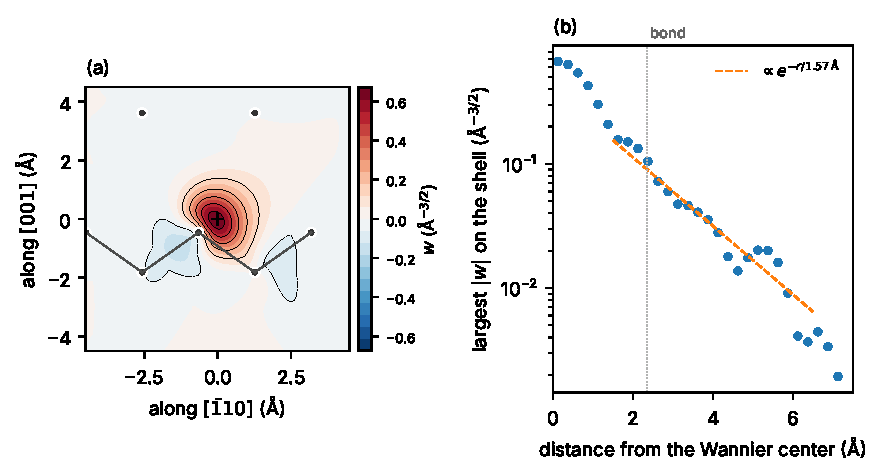
\includegraphics[width=\linewidth]{figures/ch03/fig3_11.pdf}
  \caption{A maximally localized $sp^3$ Wannier function of silicon, one of eight disentangled from the 16 lowest bands. (a)~The function on the $(110)$ plane through the atom on which it sits (cross: Wannier center; dots: atoms in the plane; lines: bonds in the plane). The plane contains the $[\bar111]$ axis of the function and the bond opposite to it. The function is real and normalized to one; red and blue are opposite signs. (b)~Largest $|w|$ on spherical shells \SI{0.25}{\angstrom} wide around the center, against distance, with an exponential fit between 2 and \SI{5.5}{\angstrom} (dashed), whose decay length is \SI{1.57}{\angstrom}. Calculation: PBE, norm-conserving SG15 pseudopotential, \SI{40}{Ry} cutoff, $a = \SI{5.431}{\angstrom}$, $6^3$ coarse grid, outer window up to \SI{12}{eV} and frozen window up to \SI{2.5}{eV} above the valence-band maximum, minimization started from $sp^3$ hybrids on both atoms pointing away from the bonds~\cite{giannozzi2017advanced,pizzi2020wannier90,hamann2013optimized,schlipf2015optimization}. The spread of each function is \SI{2.02}{\angstrom^2}; of the total $\Omega_W = \SI{16.2}{\angstrom^2}$, the gauge-invariant part $\Omega_W^{\mathrm{I}}$ is \SI{14.0}{\angstrom^2}.}
  \label{fig:3-wf}
\end{figure}

\subsection{Interpolation of the bands}

The Hamiltonian between Wannier functions follows from \cref{eq:3.6-wannier}. Since $H_{\mathrm{e}}$ does not connect different $\vect{k}$, and $\langle\psi^W_{m\vect{k}}|H_{\mathrm{e}}|\psi^W_{n\vect{k}}\rangle = \sum_{m'}U^*_{m'm}(\vect{k})\varepsilon_{m'\vect{k}}U_{m'n}(\vect{k})$, the double sum over $\vect{k}$ collapses to one:
\begin{equation}
  H^W_{mn}(\vect{R}) \equiv \langle w_{m\vect{0}}|H_{\mathrm{e}}|w_{n\vect{R}}\rangle
  = \frac1N\sum_{\vect{k}}\ee^{-\ii\vect{k}\cdot\vect{R}}\,\bigl[U^\dagger(\vect{k})\,E(\vect{k})\,U(\vect{k})\bigr]_{mn},
  \qquad E(\vect{k}) = \mathrm{diag}(\varepsilon_{n\vect{k}}) .
  \label{eq:3.6-HWR}
\end{equation}
This real-space Hamiltonian is an $N_W\times N_W$ matrix for each lattice vector. Its diagonal elements at $\vect{R} = 0$ are the on-site energies of the Wannier functions, the others are hopping integrals, and since the Wannier functions are localized it decays with $|\vect{R}|$. Its Fourier series is, by the lattice sum,
\begin{equation}
  H^W(\vect{k}) \equiv \sum_{\vect{R}}\ee^{\ii\vect{k}\cdot\vect{R}}\,H^W(\vect{R}) = U^\dagger(\vect{k})\,E(\vect{k})\,U(\vect{k}) ,
  \label{eq:3.6-HWk}
\end{equation}
a Hermitian $N_W\times N_W$ matrix whose eigenvalues are the band energies $\varepsilon_{n\vect{k}}$ and whose eigenvectors, the columns of $U^\dagger(\vect{k})$, convert the Wannier gauge back into band states~\cite[Eqs.~(98) and (99)]{marzari2012maximally}. \Cref{eq:3.6-HWk} is the tight-binding eigenvalue problem of \cref{eq:3.2-LCAO}, with orthonormal orbitals, so that $S^{\mathrm{ov}} = 1$, and with every hopping computed. In practice the Bloch states come from a plane-wave Kohn--Sham calculation (\cref{sec:3.4}) on a uniform grid; the code supplies the overlaps $M_{mn}$ and the projections $A^{\mathrm{pr}}_{mn}$, a separate program minimizes the spread, and $H^W(\vect{R})$ follows from \cref{eq:3.6-HWR} on the same grid.

The point of \cref{eq:3.6-HWk} is that its left side can be evaluated at any $\vect{k}$, not only at the points of the grid on which $H^W(\vect{R})$ was computed. On a coarse grid of $n_k = n_1n_2n_3$ points, the sum in \cref{eq:3.6-HWR} defines the coarse-grid matrix
\begin{equation*}
  \tilde H^W(\vect{R}) = \frac{1}{n_k}\sum_{j=1}^{n_k}\ee^{-\ii\vect{k}_j\cdot\vect{R}}\,H^W(\vect{k}_j) .
\end{equation*}
Inserting \cref{eq:3.6-HWk} for $H^W(\vect{k}_j)$ and using the lattice sum on the coarse grid, $n_k^{-1}\sum_j\ee^{\ii\vect{k}_j\cdot\vect{R}} = \sum_{\vect{L}_{\mathrm{sc}}}\delta_{\vect{R},\vect{L}_{\mathrm{sc}}}$, where $\vect{L}_{\mathrm{sc}} = \sum_i l_i n_i\vect{a}_i$ ($l_i$ integers) are the lattice vectors of the supercell that the coarse grid makes periodic, we find
\begin{equation}
  \tilde H^W(\vect{R}) = \sum_{\vect{L}_{\mathrm{sc}}}H^W(\vect{R} + \vect{L}_{\mathrm{sc}}) .
  \label{eq:3.6-alias}
\end{equation}
The coarse grid does not lose the hoppings; it folds them onto one supercell, so that a hopping to $\vect{R} + \vect{L}_{\mathrm{sc}}$ is added to the hopping to $\vect{R}$. This aliasing is the only error of the interpolation. Suppose $H^W(\vect{R})$ vanishes beyond some range $R_{\mathrm{max}}$, and the supercell is large enough that every $\vect{R}$ with $|\vect{R}| \le R_{\mathrm{max}}$ lies inside its Wigner--Seitz cell. Then at most one term of \cref{eq:3.6-alias} is nonzero for each $\vect{R}$ of that cell, and $\tilde H^W(\vect{R}) = H^W(\vect{R})$ there. A lattice vector on the boundary of the Wigner--Seitz cell belongs to two or more cells; its term is shared among its images with weights that add up to one, which restores the same result.
\begin{keyresult}[Exactness of Wannier interpolation]
If the real-space Hamiltonian $H^W(\vect{R})$ has finite range $R_{\mathrm{max}}$, and the supercell of the coarse grid contains the sphere of radius $R_{\mathrm{max}}$ in its Wigner--Seitz cell, then
\begin{equation}
  \sum_{\vect{R}\in\mathrm{WS}}\ee^{\ii\vect{k}\cdot\vect{R}}\,\tilde H^W(\vect{R}) = H^W(\vect{k}) \quad\text{for every }\vect{k},
  \label{eq:3.6-exact}
\end{equation}
and its eigenvalues are the exact bands $\varepsilon_{n\vect{k}}$, on the coarse grid and between its points. The sum runs over the lattice vectors of the Wigner--Seitz supercell, with fractional weights on its boundary.
\end{keyresult}
Real Wannier functions are not of finite range. They decay exponentially, and so does $H^W(\vect{R})$. The error of the interpolation is then the aliased tail of \cref{eq:3.6-alias}, of the size of $H^W$ at a distance of half a supercell, and it falls exponentially as the coarse grid is refined; \cref{we:3-w1d} shows both behaviors in a model. The gauge enters at this point. The bands at the grid points do not depend on $U(\vect{k})$, but the range of $H^W(\vect{R})$ does, and the most localized Wannier functions make the shortest-ranged Hamiltonian and the fastest convergence. With disentanglement, the interpolated bands are exact only inside the frozen window; outside it they are the bands of the selected subspace.

\Cref{fig:3-wint} applies this to silicon, where the convergence is slower than the size of the Wannier functions suggests. The four bond-centered functions of the valence bands have a total spread of \SI{7.58}{\angstrom^2} on a $6^3$ grid. Interpolated from $4^3$, $6^3$ and $8^3$ grids, their bands deviate from a direct calculation by at most 350, 120 and \SI{51}{meV}, about a factor 2.5 for every two added points per direction. The reason is visible in $H^W(\vect{R})$. Its elements fall to \SI{0.02}{eV} at \SI{5.4}{\angstrom} in most directions, but along the twelve $\langle110\rangle$ directions, in which the bonds of the diamond structure form zigzag chains, they are \SI{0.12}{eV} two lattice vectors away (\SI{7.7}{\angstrom}) and \SI{0.03}{eV} three away (\SI{11.5}{\angstrom}). These are the hoppings that the coarse grids fold back. For the eight $sp^3$ functions on the $8^3$ grid, the valence bands are within \SI{40}{meV} and the conduction bands below \SI{1.5}{eV} within \SI{84}{meV}. The largest error is near the conduction minimum, which lies between the grid points, and calculations of rates use denser coarse grids for the conduction bands for this reason.

Derivatives follow analytically. Differentiating \cref{eq:3.6-HWk} analytically, $\nabla_{\vect{k}}H^W(\vect{k}) = \sum_{\vect{R}}\ii\vect{R}\,\ee^{\ii\vect{k}\cdot\vect{R}}H^W(\vect{R})$, and by the Hellmann--Feynman argument of \cref{eq:3.2-vg} its diagonal elements in the band basis are the group velocities. The interband velocities need more. By \cref{eq:3.2-dudk}, $\vect{v}_{mn} = (\varepsilon_{n\vect{k}} - \varepsilon_{m\vect{k}})\langle u_{m\vect{k}}|\nabla_{\vect{k}}u_{n\vect{k}}\rangle$ for $m \ne n$, and the overlap on the right is interpolated from the matrix elements of $\vect{r}$ between Wannier functions, \cref{eq:3.6-blount}, rotated with the same $U(\vect{k})$~\cite[Eqs.~(106)--(109)]{marzari2012maximally}; the Hamiltonian alone would treat the Wannier functions as point-like orbitals.

\begin{figure}[tbp]
  \centering
  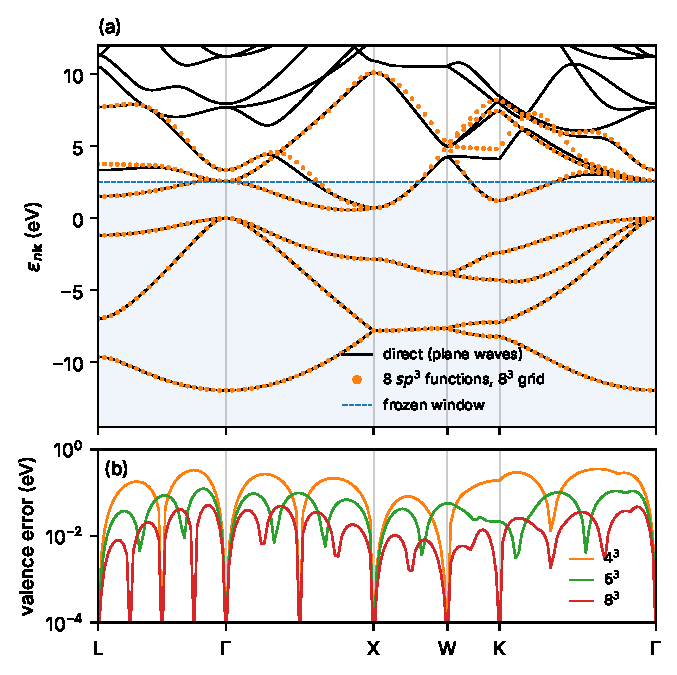
\includegraphics[width=0.78\linewidth]{figures/ch03/fig3_12.pdf}
  \caption{Wannier interpolation of the bands of silicon. (a)~Bands computed directly in plane waves at each point of the path (lines) and interpolated from the eight $sp^3$ Wannier functions of \cref{fig:3-wf}, built on an $8^3$ coarse grid (dots), relative to the valence-band maximum. Inside the frozen window (shaded, up to \SI{2.5}{eV}) the Wannier bands follow the four valence and the lowest conduction bands; above it they follow the selected subspace, not the true bands, and the higher bands (lines without dots) are outside the Wannier manifold. (b)~Largest error of the four valence bands interpolated from four bond-centered Wannier functions, an isolated group, for coarse grids of $4^3$, $6^3$ and $8^3$ points. It vanishes at $\mathrm{\Gamma}$, X and L, which lie on all three grids. PBE calculation as in \cref{fig:3-wf}; its gap, \SI{0.557}{eV} at $0.843\,(2\pi/a)$ along $\mathrm{\Gamma}$X, is the Kohn--Sham gap of \cref{sec:3.4}, not the measured \SI{1.17}{eV}.}
  \label{fig:3-wint}
\end{figure}

\subsection{One gauge for all interpolated quantities}

Any operator that conserves crystal momentum interpolates the same way. If $O_{mn}(\vect{k}) = \langle\psi_{m\vect{k}}|O|\psi_{n\vect{k}}\rangle$ is known on the grid, its Wannier-gauge form $U^\dagger(\vect{k})O(\vect{k})U(\vect{k})$ is transformed to real space as in \cref{eq:3.6-HWR}, summed back at the new $\vect{k}$ as in \cref{eq:3.6-HWk}, and rotated into the band basis with the eigenvectors of $H^W(\vect{k})$ at that point. Vertices that change the crystal momentum, the density vertex $\rho_{mn}(\vect{k},\vect{q})$ and the electron--phonon vertex, carry one gauge matrix at each end, $U^\dagger(\vect{k} + \vect{q})\,\rho(\vect{k},\vect{q})\,U(\vect{k})$, and are interpolated in the same way (\cref{eq:E.5-ginterp}). The step back into the band basis uses the eigenvectors of the interpolated Hamiltonian. As a result, the band index of an interpolated vertex refers to the interpolated bands only if the vertex and the Hamiltonian were rotated into the Wannier gauge with the same $U(\vect{k})$. That is the rule of \cref{app:A.5}. Suppose $O(\vect{k})$ was computed from states that differ from those behind $U(\vect{k})$ by phases, $\psi_{m\vect{k}} \to \ee^{\ii\theta_m(\vect{k})}\psi_{m\vect{k}}$, as two independent diagonalizations produce. With $D(\vect{k}) = \mathrm{diag}\,\ee^{\ii\theta_m(\vect{k})}$, the matrix that is transformed is $U^\dagger D^\dagger OD\,U$, the operator in the gauge $DU$. That gauge jumps at random from point to point, its real-space form does not decay, and \cref{eq:3.6-alias} folds an unbounded tail onto the supercell. The interpolated matrix elements between the grid points are then wrong by amounts as large as the elements themselves. At the grid points the moduli $|O_{mn}|$ of nondegenerate bands survive, because there the error is only a phase. A check made on the grid does not reveal it. For degenerate bands, such as the valence-band maximum of silicon at $\mathrm{\Gamma}$, $D$ is a unitary mixing and even the moduli are lost. The interpolated energies carry no trace of the mismatch, since $H^W$ was rotated with its own states.

A first-order rate contains only $|\rho_{mn}|^2$ between fixed bands, so a gauge mismatch spoils it between the grid points but not on them. A second-order amplitude is not protected even on the grid. It sums products such as $g_{cm\nu}\rho_{mv}$ over the intermediate band $m$ (\cref{sec:6.5}), and the phase of band $m$ cancels between the two factors only if both were built from the same state. Every quantity that enters one amplitude is therefore computed from one set of wavefunctions and rotated with one set of gauge matrices. The density vertex depends on the momentum transfer $\vect{q}$, which is a parameter, not a crystal momentum of the grid, and at $q \sim q_0$ the factor $\ee^{\ii\vect{q}\cdot\vect{r}}$ varies over a single Wannier function. Its real-space form must then be built separately for each $\vect{q}$.

\begin{workedexample}{A two-band chain interpolated from a coarse grid}\label{we:3-w1d}
A chain of lattice constant $a$ has two orthonormal orbitals per cell, on sites a and b, with on-site energies $E_{\mathrm{a}} = -E_{\mathrm{b}} = \SI{0.5}{eV}$, a hopping matrix element $-t_{\mathrm{hop}}$ between the two sites of a cell and $-t'_{\mathrm{hop}}$ between site a of one cell and site b of the cell to its left, with $t_{\mathrm{hop}} = \SI{2.0}{eV}$ and $t'_{\mathrm{hop}} = \SI{1.0}{eV}$. The numbers are illustrative, not fitted to a material. In the basis of Bloch sums of the two orbitals, \cref{eq:3.2-HS} gives
\begin{gather*}
  H(k) = \begin{pmatrix} E_{\mathrm{a}} & -t_{\mathrm{hop}} - t'_{\mathrm{hop}}\ee^{-\ii ka} \\ -t_{\mathrm{hop}} - t'_{\mathrm{hop}}\ee^{\ii ka} & -E_{\mathrm{a}} \end{pmatrix}, \\
  \varepsilon_{\pm,k} = \pm\bigl(E_{\mathrm{a}}^2 + t_{\mathrm{hop}}^2 + t'^2_{\mathrm{hop}} + 2t_{\mathrm{hop}}t'_{\mathrm{hop}}\cos ka\bigr)^{1/2} .
\end{gather*}
The two bands span $\pm\SI{1.118}{eV}$ to $\pm\SI{3.041}{eV}$, with a gap of \SI{2.236}{eV} at $k = \pi/a$. We treat the model as a code would. On a grid of $n_k$ points $k_j = 2\pi j/(n_ka)$ we diagonalize $H(k_j)$ and give each eigenvector a random phase. We then build the gauge by projection, \cref{eq:3.6-projection}, on the two orbitals, and compute $\tilde H^W(R)$ on the Wigner--Seitz supercell, $R = -\lfloor n_k/2\rfloor a, \dots, \lfloor n_k/2\rfloor a$, with weight $\frac12$ on the two end points when $n_k$ is even. Finally we diagonalize the interpolated $H^W(k)$ at 2001 points between $-\pi/a$ and $\pi/a$ and compare with $\varepsilon_{\pm,k}$.

\emph{Two Wannier functions.} For the pair of bands the projection returns $U(k_j) = C^\dagger(k_j)$, with $C$ the eigenvector matrix, and the random phases cancel. The Wannier functions are the two orbitals themselves, and $H^W(R)$ has range $a$: on-site energies and $-t_{\mathrm{hop}}$ at $R = 0$, $-t'_{\mathrm{hop}}$ at $R = \pm a$, nothing beyond. The exactness condition of \cref{eq:3.6-exact} requires the supercell to hold $R = -a, 0, a$ inside its Wigner--Seitz cell, that is $n_k \ge 3$. With $n_k = 3$, 4 and 6 the largest band error is \SIrange{1e-15}{3e-15}{eV}, rounding error. With $n_k = 2$ the hoppings to $R = +a$ and $R = -a$ fall on the same boundary point, they are not equal (one couples a to b, the other b to a), and the error is \SI{0.24}{eV}.

\emph{One Wannier function.} The lower band alone is an isolated band, and its Wannier function is a combination of both orbitals in many cells. Its $H^W(R)$ is the set of Fourier coefficients of $\varepsilon_{-,k}$, which do not depend on the gauge. It decays as $|R|^{-3/2}\ee^{-|R|/\xi_W}$, where $1/\xi_W$ is the distance of the nearest branch point of $\varepsilon_{-,k}$ from the real axis, at $\cos ka = -(E_{\mathrm{a}}^2 + t_{\mathrm{hop}}^2 + t'^2_{\mathrm{hop}})/(2t_{\mathrm{hop}}t'_{\mathrm{hop}}) = -1.3125$, so that $a/\xi_W = \mathrm{arccosh}\,1.3125 = 0.771$. In numbers, $|H^W(R)| = 2.19$, 0.468, 0.0525 and \SI{0.0120}{eV} for $R/a = 0$ to 3, and the ratio of successive values approaches $(R/(R+1))^{3/2}\ee^{-a/\xi_W}$, with $\ee^{-a/\xi_W} = 0.462$. The interpolation error is now never zero. It is \SI{51}{meV} for $n_k = 4$, \SI{4.7}{meV} for 8, \SI{0.64}{meV} for 12 and \SI{2.4}{\micro eV} for 24, approaching a factor $\ee^{-a/2\xi_W} = 0.68$ per added grid point, as the aliased tail at half a supercell predicts; at small $n_k$ the power-law factor makes the fall somewhat faster. A tolerance of \SI{1}{meV} needs 12 points.

\emph{One gauge.} For the gauge test we take the matrix $\partial H/\partial k$ of the model, whose band-diagonal elements are the group velocities, and interpolate its interband element $|(\partial H/\partial k)_{+-}|$, which ranges between 0.27 and $1.00\,\mathrm{eV}\,a$ along the zone. With $n_k = 6$ we compute it in the band basis of one set of random phases. Rotated into the Wannier gauge with the eigenvectors of that set, it interpolates to within $10^{-15}\,\mathrm{eV}\,a$ everywhere. Rotated instead with the eigenvectors of a second, independent set, which describe the same states with other phases, it is correct in modulus at the six grid points and off between them by amounts that depend on the random phases, up to 0.3 to $0.8\,\mathrm{eV}\,a$ in different draws, as large as the matrix element itself. The interpolated bands are exact in both cases.
\end{workedexample}

The interpolated energies, velocities and vertices on fine grids are the inputs of the phonon-assisted rates of \cref{sec:6.5,sec:13.3}. Wannier functions make the electron--phonon vertex as short-ranged as the Hamiltonian, which lets those grids be filled (\cref{sec:6.2}), except for the long-range dipole part of polar crystals, which is split off analytically (\cref{app:E.5}).
